\section{Measurement}
\label{section:measurement}


\subsection{\bf Experiment Setup}

Fill experiment setup here.

\subsection{\bf Workload Description}
We run three kinds of workloads and capture the pcap trace on each machine.
(1) Write files to HDFS
We first run one HDFS client which writes a 1GB file into HDFS on each of the 6 machines at the same time. Each client will write 4KB at one time until it reaches 1GB. HDFS block size is set to 64MB and replica number is 3.

(2) Read
We then run four HDFS clients at the same time, one on each slave node (4 nodes in total). Each client will read the 1GB file we just generated on that slave node. HDFS block size is set to 64MB and replica number is 3.

(3) Change the number of replica on the fly
We then change the number of replicas from 3 to 4 for one 1GB file we just generated in HDFS with command "hadoop dfs -setrep -w 4 the_path_of_the_file"

\subsection{\bf Flow Size Analysis}
We have analyzed the flow size for each specific type of flows, and the results are shown in figure \ref{fig:read_size}, \ref{fig:write_size} and \ref{fig:replica_size}.



%\begin{comment}
%\begin{figure*}[htb]
%\begin{figure*}[!ht]
%\label{fig:read_size}
%\centering	
%   \begin{tabular}{@{}cc@{}}
%	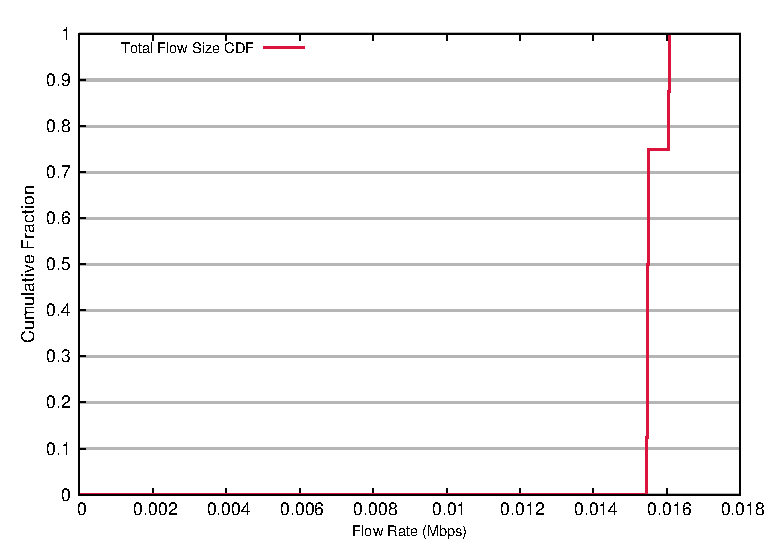
\includegraphics[width=.55\textwidth]{figures/4read/24_28_flow_size.eps} &
%	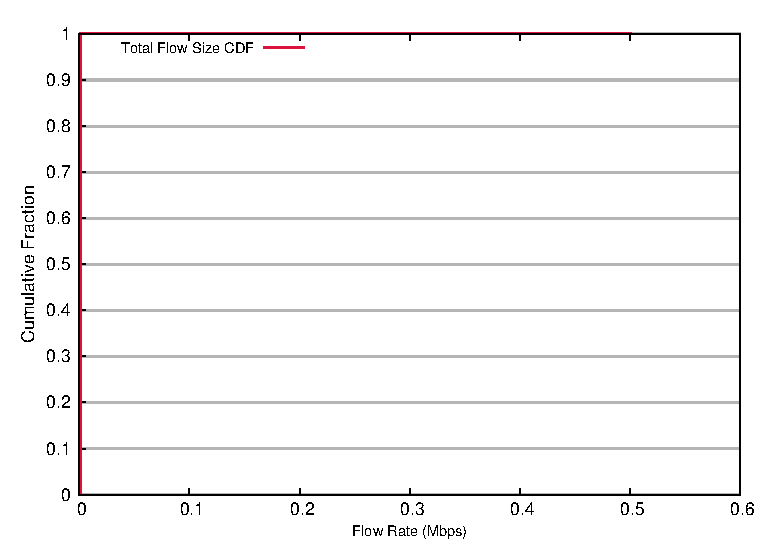
\includegraphics[width=.55\textwidth]{figures/4read/8_12_flow_size.eps}  \\
%	\multicolumn{2}{c}{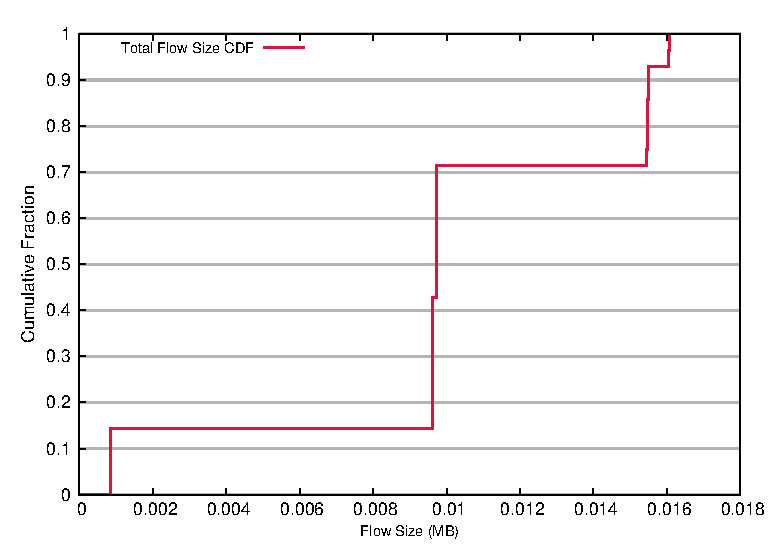
\includegraphics[width=.73\textwidth]{figures/4read/flow_size.eps}}
%    \end{tabular}
%\caption{Read Flow Size Distribution}
%\end{figure*}
%\end{comment}

\begin{figure*}[!ht]
\label{fig:read_size}
\centering
  \begin{subfigure}[b]{.45\linewidth}
   \centering
	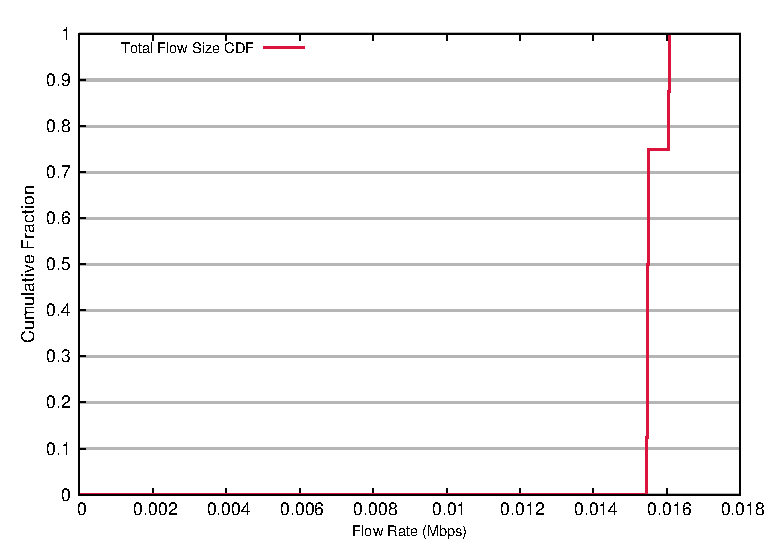
\includegraphics[width=.99\textwidth]{figures/4read/24_28_flow_size.eps} 
	\caption{RPC between Client and DataNodes}\label{fig:read_size:rpc}
   \end{subfigure}%
  \begin{subfigure}[b]{.45\linewidth}
   \centering
	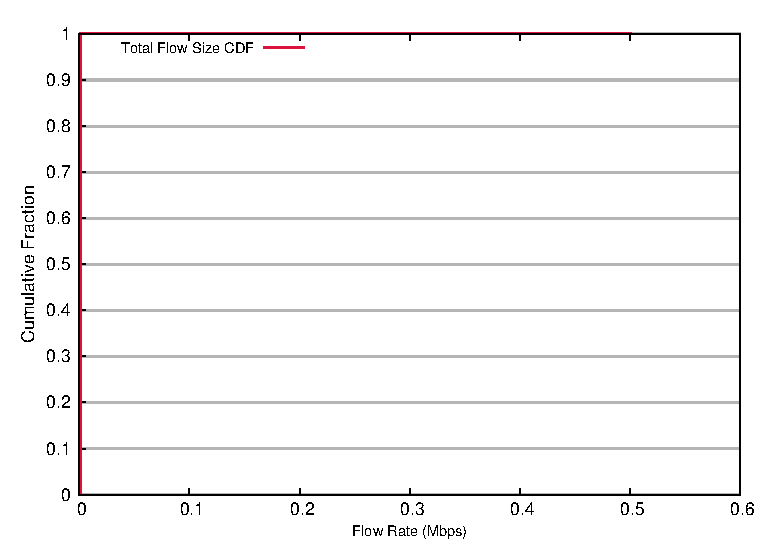
\includegraphics[width=.99\textwidth]{figures/4read/8_12_flow_size.eps} 
	\caption{Should have read data transfer here}\label{fig:read_size:fixme}
   \end{subfigure} \\%
  \begin{subfigure}[b]{.75\linewidth}
   \centering
	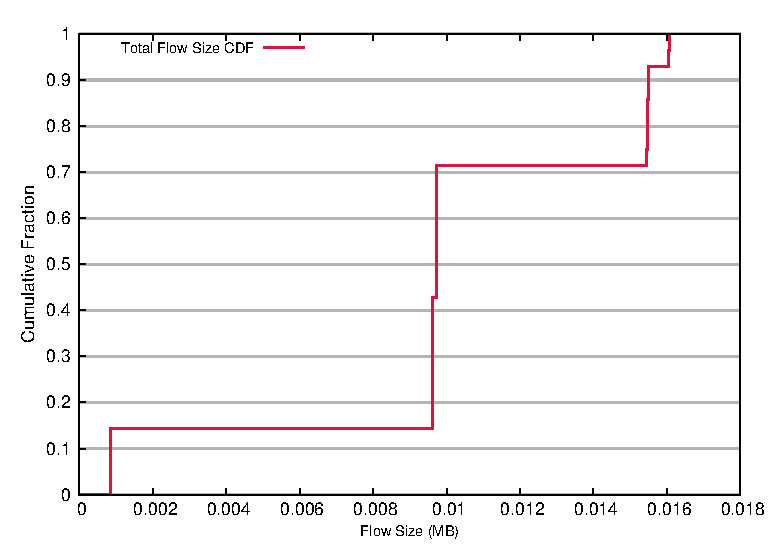
\includegraphics[width=.99\textwidth]{figures/4read/flow_size.eps}
	\caption{All Traffic}\label{fig:read_size:all}
   \end{subfigure}%
\caption{Read Flow Size Distribution}
\end{figure*}

FXIME: read workload doesn't make sense here, needs to fix it.


\begin{figure*}[!ht]
\label{fig:write_size}
\centering
  \begin{subfigure}[b]{.45\linewidth}
   \centering
	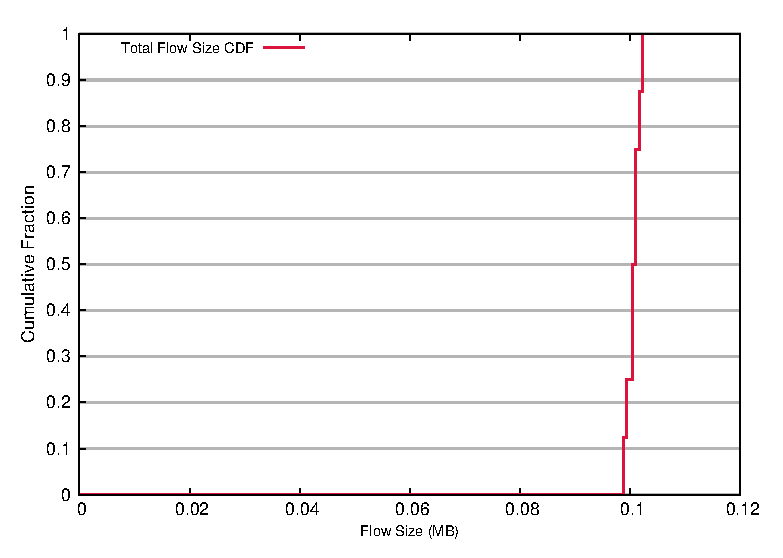
\includegraphics[width=.99\textwidth]{figures/6writes/24_28_type_flow_size.eps} 
	\caption{DataNodes RPC with NameNode}\label{fig:write_size:dn_rpc}
   \end{subfigure}%
  \begin{subfigure}[b]{.45\linewidth}
   \centering
	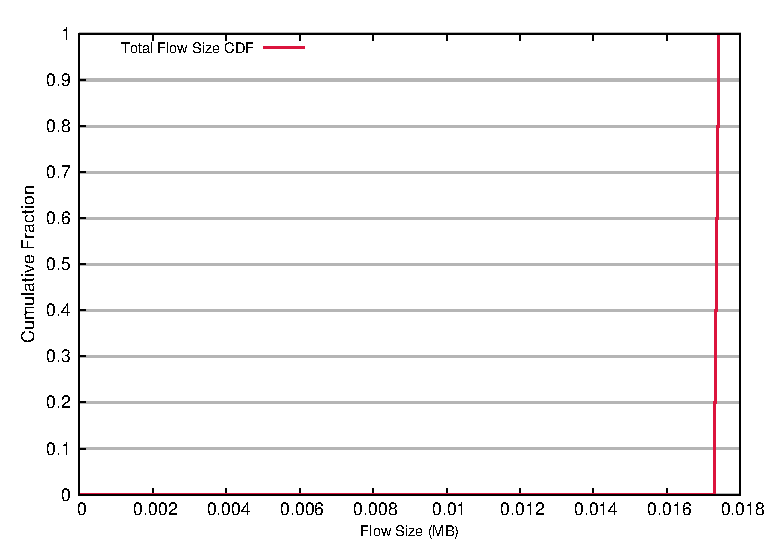
\includegraphics[width=.99\textwidth]{figures/6writes/24_28_20_16_type_flow_size.eps} 
	\caption{Client and DataNodes RPC with NameNode}\label{fig:write_size:dc_rpc}
   \end{subfigure} \\%
  \begin{subfigure}[b]{.45\linewidth}
   \centering
	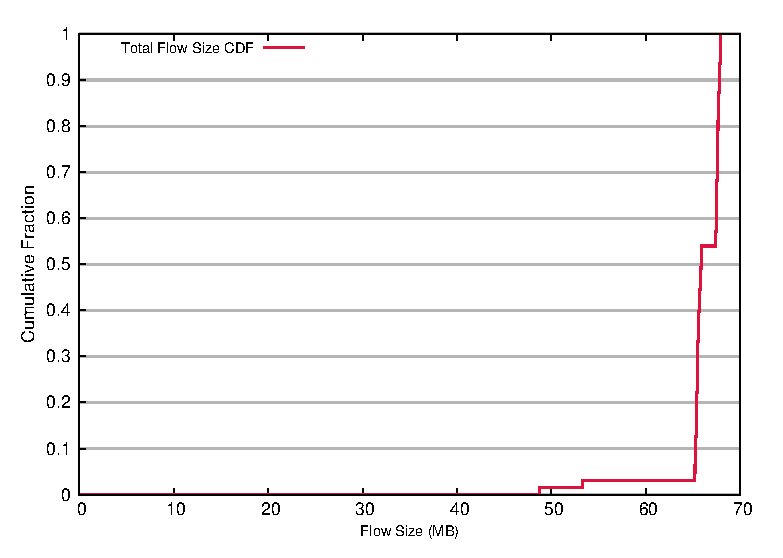
\includegraphics[width=.99\textwidth]{figures/6writes/36_44_type_flow_size.eps} 
	\caption{Pipelined Writes between DataNodes}\label{fig:write_size:pipe_write}
   \end{subfigure} %
  \begin{subfigure}[b]{.45\linewidth}
   \centering
	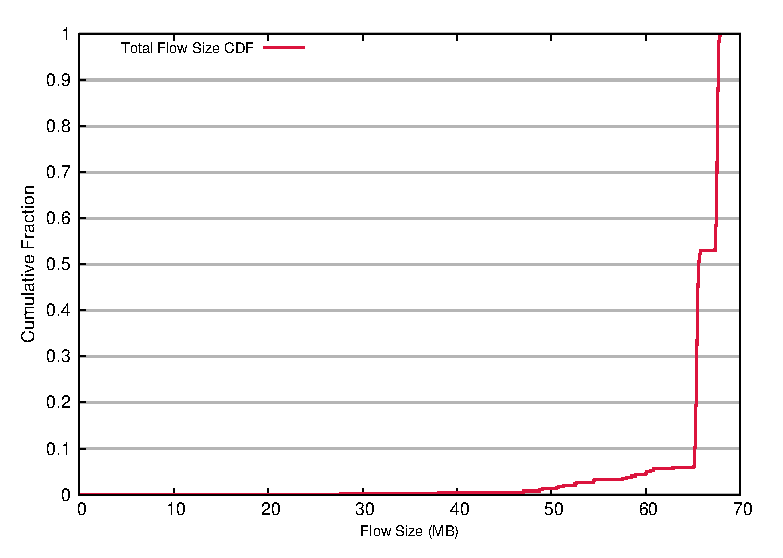
\includegraphics[width=.99\textwidth]{figures/6writes/32_36_type_flow_size.eps} 
	\caption{Client Data Transfer to DataNodes}\label{fig:write_size:client_write}
   \end{subfigure} \\%
  \begin{subfigure}[b]{.75\linewidth}
   \centering
	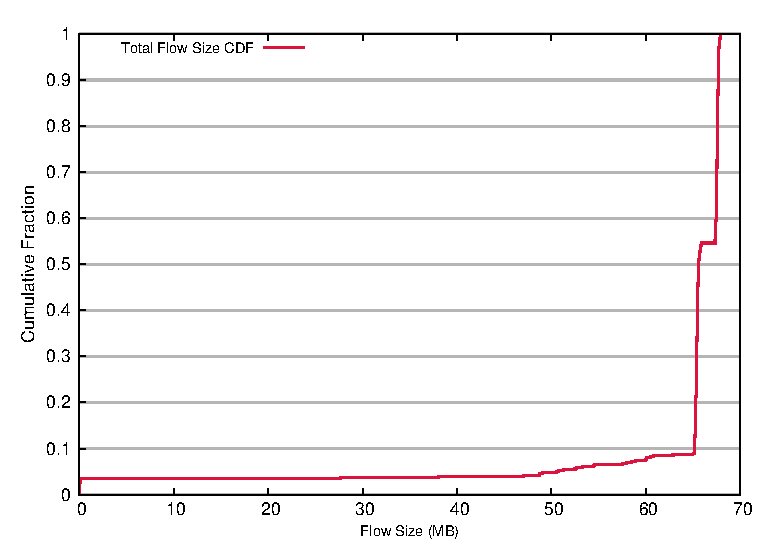
\includegraphics[width=.99\textwidth]{figures/6writes/flow_size.eps}
	\caption{All Traffic}\label{fig:write_size:all}
   \end{subfigure}%
\caption{Write Flow Size Distribution}
\end{figure*}


The flow size distribution of the write workload shown in figure \ref{fig:write_size} revealed some information about HDFS's internal operation. We can see that there are twon kinds of flows, RPC flows, which typically has very small data transferred; and data transfer flows, including the pipelined data transfer between data nodes and the data client writes to the datanodes, which is around 65 MB. This is in compliance with the fact that HDFS has separate flows for RPC calls/responses and data transfers; and data transfer is done in the unit of blocks, which is 64 MB in our configuration. We could also see that less than 5\% of the flows are used for RPC calls to transfer control information, while the majority of the flows are used for data transfer, which is as expected. 

\begin{figure*}[!ht]
\label{fig:replica_size}
\centering
  \begin{subfigure}[b]{.45\linewidth}
   \centering
	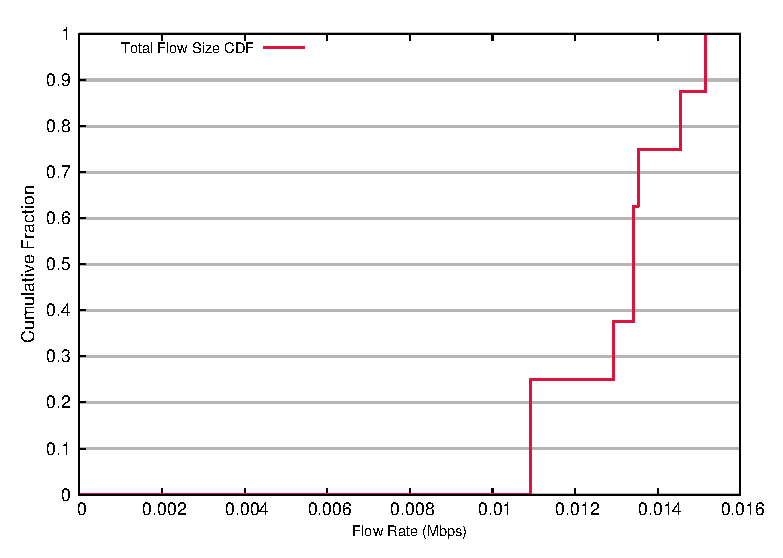
\includegraphics[width=.99\textwidth]{figures/replica_change/24_28_flow_size.eps} 
	\caption{DataNodes RPC with NameNode}\label{fig:replica_size:rpc}
   \end{subfigure}%
  \begin{subfigure}[b]{.45\linewidth}
   \centering
	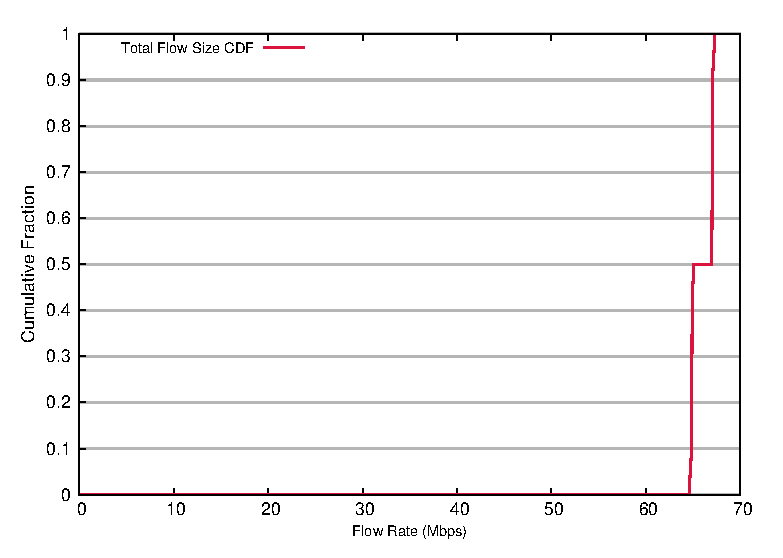
\includegraphics[width=.99\textwidth]{figures/replica_change/36_32_flow_size.eps} 
	\caption{Pipelined Writes between DataNodes}\label{fig:replica_size:pipe_write}
   \end{subfigure} \\%
  \begin{subfigure}[b]{.75\linewidth}
   \centering
	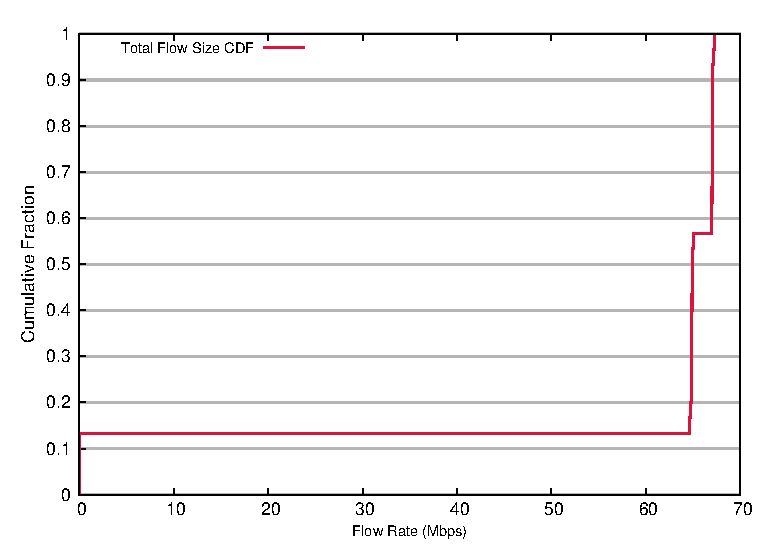
\includegraphics[width=.99\textwidth]{figures/replica_change/flow_size.eps}
	\caption{All Traffic}\label{fig:read_size:all}
   \end{subfigure}%
\caption{Replciation Level Change Flow Size Distribution}
\end{figure*}

The flow size distribution of the replication level change workload in figure \ref{fig:replica_size} exihibed the same characteristics, except for that we have less data transfers and relatively more control messages. 


\subsection{\bf Flow Duration Analysis}
The flow duration distributions for each kind of workloads are shown in figure \ref{fig:read_duration}, \ref{fig:write_duration} and \ref{fig:replica_duration}.

\begin{figure*}[!htpb]
\centering
  \begin{subfigure}[b]{.45\linewidth}
   \centering
	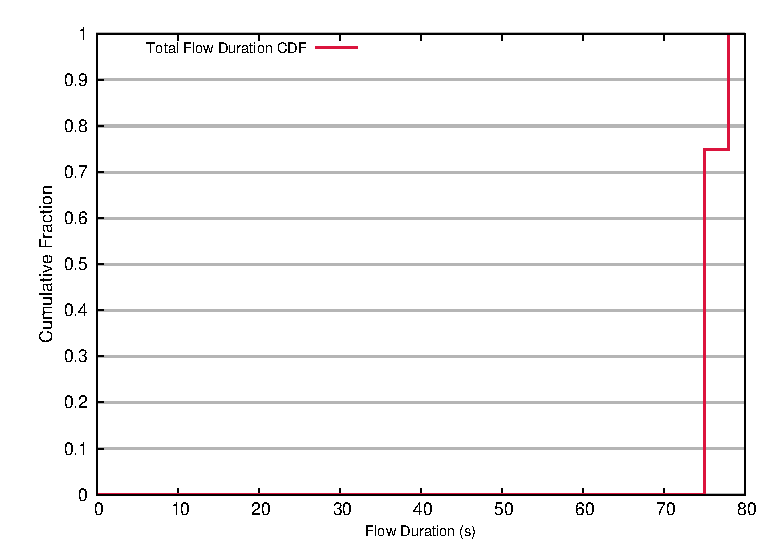
\includegraphics[width=.99\textwidth]{figures/4read/24_28_type_duration.eps} 
	\caption{RPC between Client and DataNodes}\label{fig:read_duration:rpc}
   \end{subfigure}%
  \begin{subfigure}[b]{.45\linewidth}
   \centering
	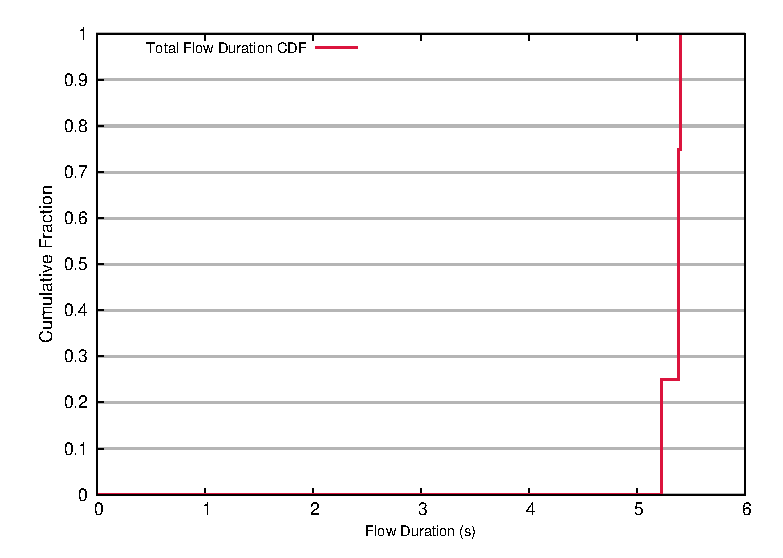
\includegraphics[width=.99\textwidth]{figures/4read/24_28_20_16_type_duration.eps} 
	\caption{Client and DataNodes RPC with NameNode}\label{fig:read_duration:nn_rpc}
   \end{subfigure} \\%
  \begin{subfigure}[b]{.55\linewidth}
   \centering
	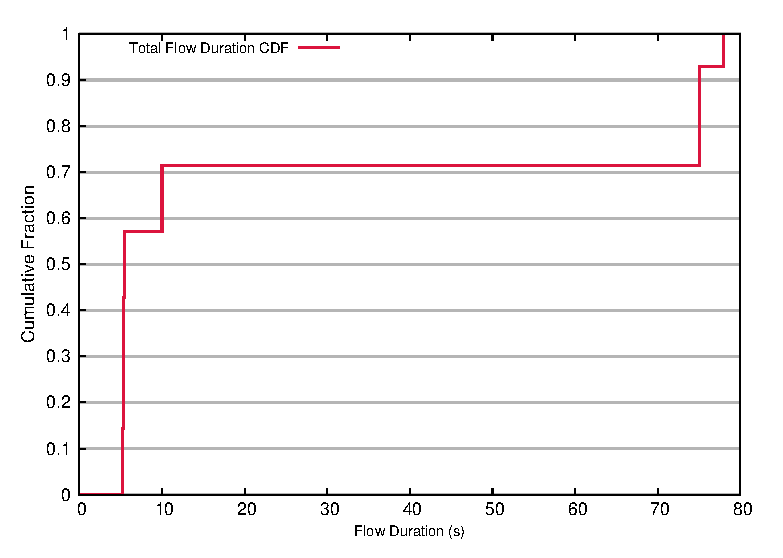
\includegraphics[width=.99\textwidth]{figures/4read/flow_duration.eps}
	\caption{All Traffic}\label{fig:read_duration:all}
   \end{subfigure}%
\caption{Read Flow Duration Distribution}
\label{fig:read_duration}
\end{figure*}

Again, we could see in figure \ref{fig:read_duration} that for the read workloads, almost all the flows are long lived RPC flows.

\begin{figure*}[!htbp]
\centering
  \begin{subfigure}[b]{.45\linewidth}
   \centering
	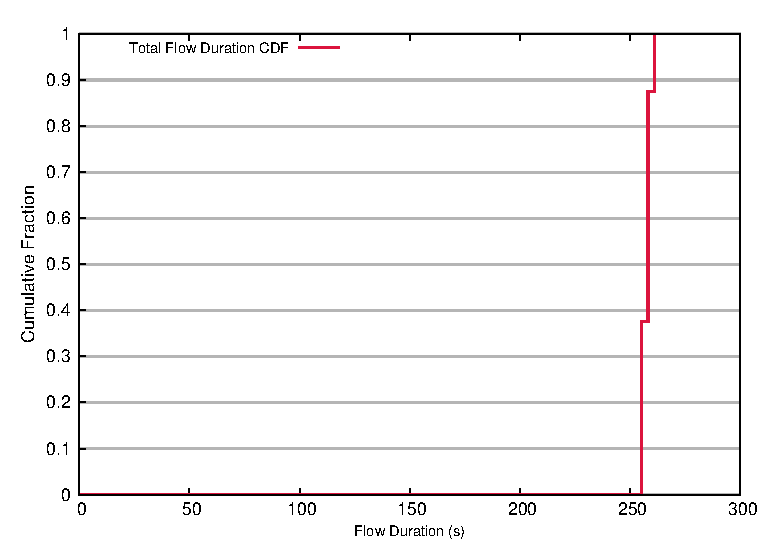
\includegraphics[width=.99\textwidth]{figures/6writes/24_28_type_flow_duration.eps} 
	\caption{DataNodes RPC with NameNode}\label{fig:write_duration:dn_rpc}
   \end{subfigure}%
  \begin{subfigure}[b]{.45\linewidth}
   \centering
	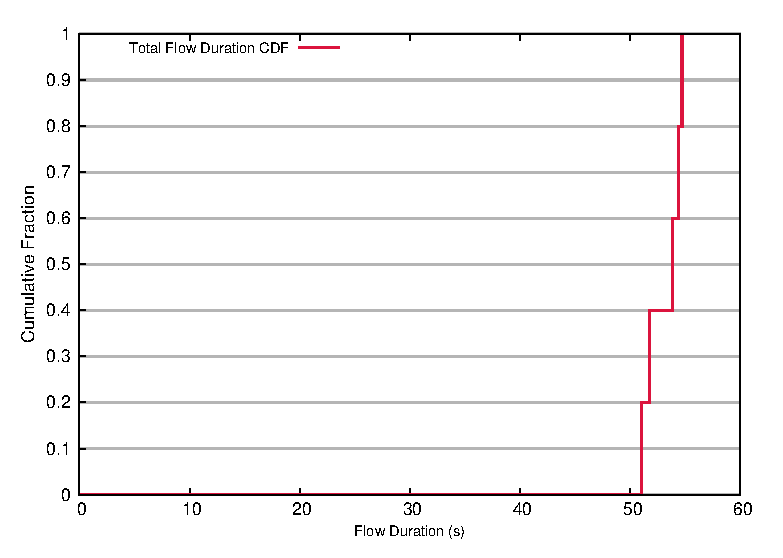
\includegraphics[width=.99\textwidth]{figures/6writes/24_28_20_16_type_flow_duration.eps} 
	\caption{Client and DataNodes RPC with NameNode}\label{fig:write_duration:dc_rpc}
   \end{subfigure} \\%
  \begin{subfigure}[b]{.45\linewidth}
   \centering
	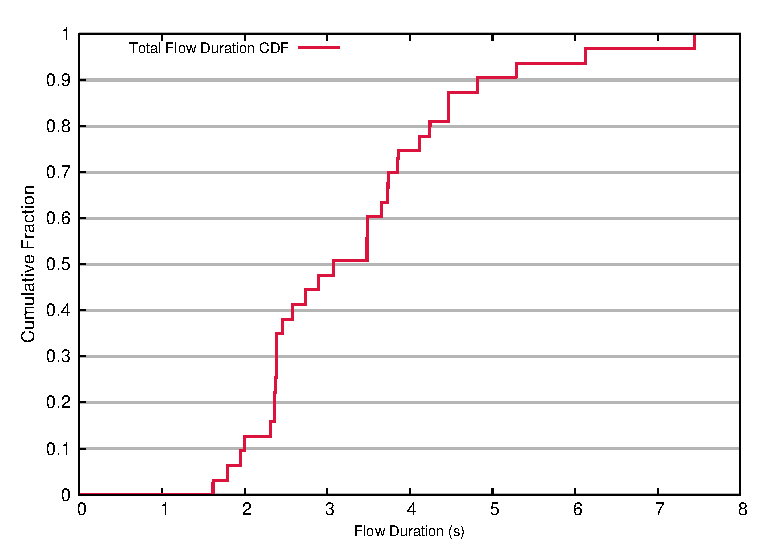
\includegraphics[width=.99\textwidth]{figures/6writes/36_44_type_flow_duration.eps} 
	\caption{Pipelined Writes between DataNodes}\label{fig:write_duration:pipe_write}
   \end{subfigure} %
  \begin{subfigure}[b]{.45\linewidth}
   \centering
	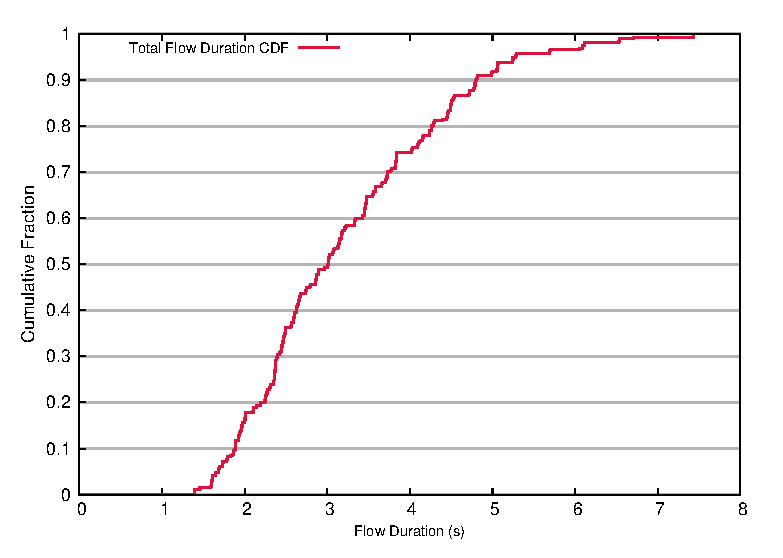
\includegraphics[width=.99\textwidth]{figures/6writes/32_36_type_flow_duration.eps} 
	\caption{Client Data Transfer to DataNodes}\label{fig:write_duration:client_write}
   \end{subfigure} \\%
  \begin{subfigure}[b]{.45\linewidth}
   \centering
	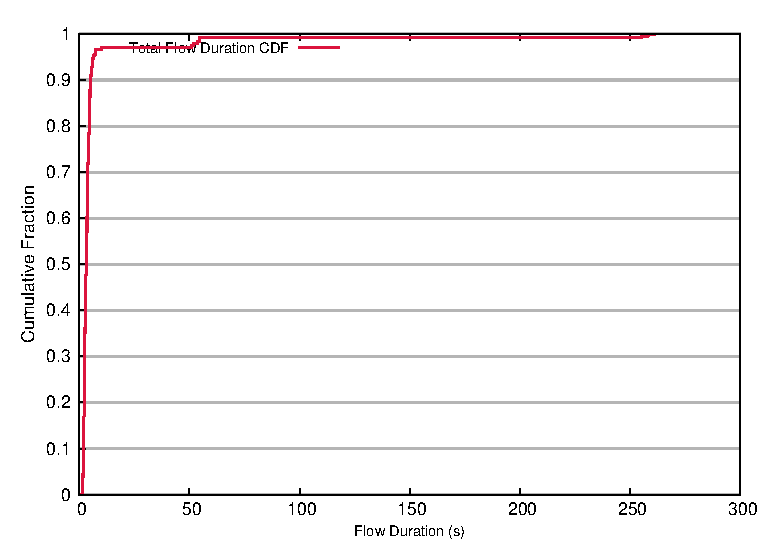
\includegraphics[width=.99\textwidth]{figures/6writes/flow_duration.eps}
	\caption{All Traffic}\label{fig:write_duration:all}
   \end{subfigure}%
  \begin{subfigure}[b]{.45\linewidth}
   \centering
	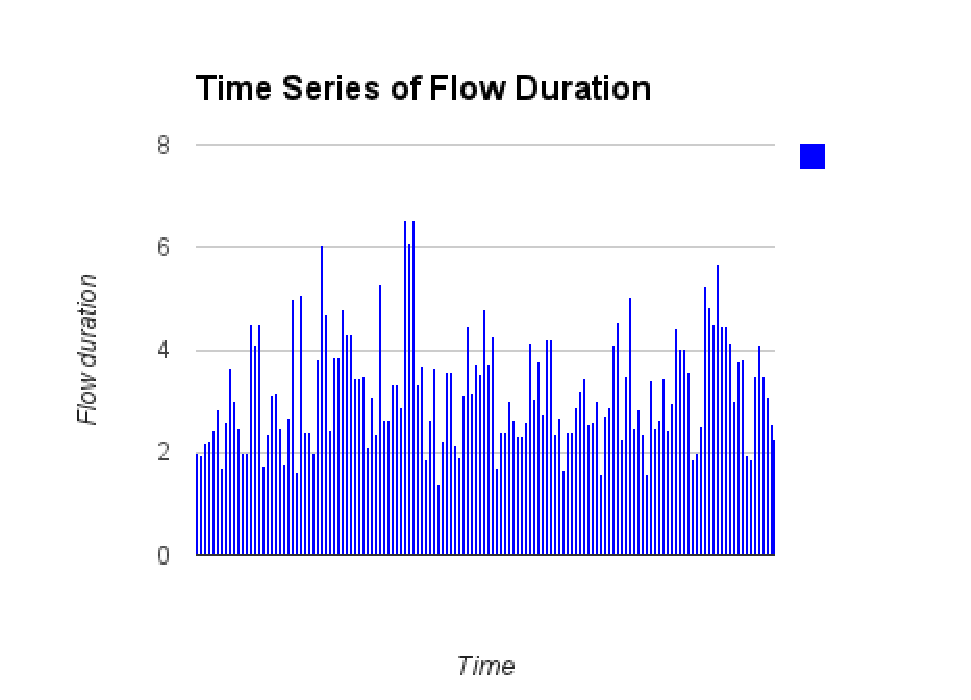
\includegraphics[width=.99\textwidth]{figures/6writes/flow_duration_time_series.eps}
	\caption{Time Series of All Traffic}\label{fig:write:time_series}
   \end{subfigure}%
\caption{Write Flow Duration Distribution}
\label{fig:write_duration}
\end{figure*}

For the write workload, we can again see the radical differences between RPC calls/responds flows, which are long lived and shared among multiple RPC calls; and data transfer flows, which transfers one block of file data in HDFS in its lifetime. However, we have noticed that the data transfer flows' duration spans a wide range, from less than 2 seconds to more than seven seconds, even though all of them transfer the same amount of data. In order to determine whether this is caused by network congestion or any hotspots within the network, we looked the flow duration on each link of the network, and found that this distribution is not dependent on the network location. Actually flows between any two nodes in our network exhibit the similar duration distribution (results omitted in the interest of space). The time series of the flow duration is also shown in figure \ref{fig:write:time_series}, and we could see periodic spike in the flow duration. We think it could be related to the network condition, but no further information is available to investigate the cause of it.

\begin{figure*}[!htbp]
\centering
  \begin{subfigure}[b]{.45\linewidth}
   \centering
	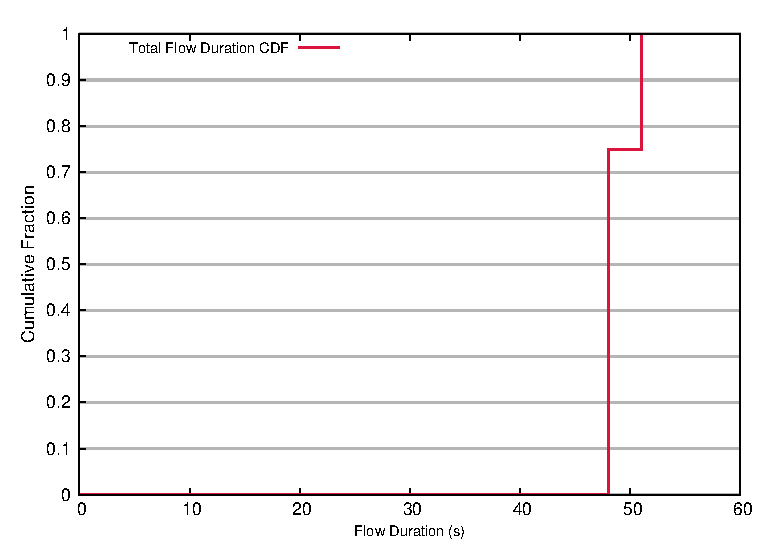
\includegraphics[width=.99\textwidth]{figures/replica_change/24_28_flow_duration.eps} 
	\caption{DataNodes RPC with NameNode}\label{fig:replica_duration:rpc}
   \end{subfigure}%
  \begin{subfigure}[b]{.45\linewidth}
   \centering
	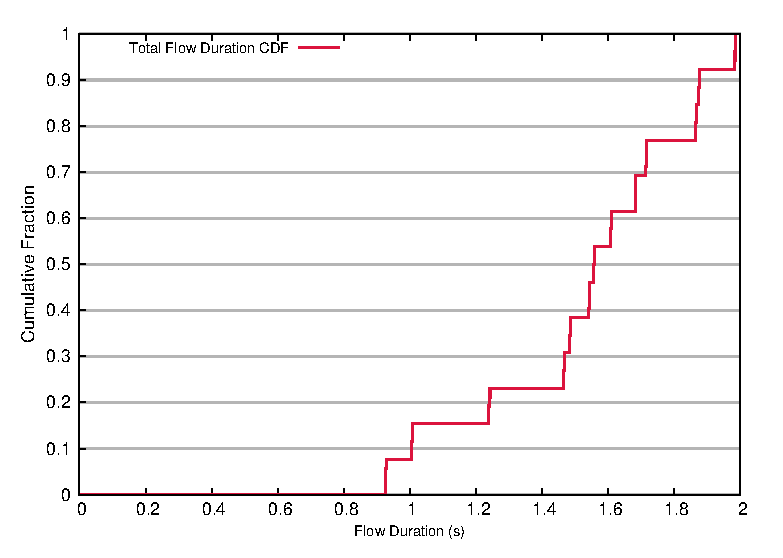
\includegraphics[width=.99\textwidth]{figures/replica_change/36_32_flow_duration.eps} 
	\caption{Pipelined Writes between DataNodes}\label{fig:replica_duration:pipe_write}
   \end{subfigure} \\%
  \begin{subfigure}[b]{.55\linewidth}
   \centering
	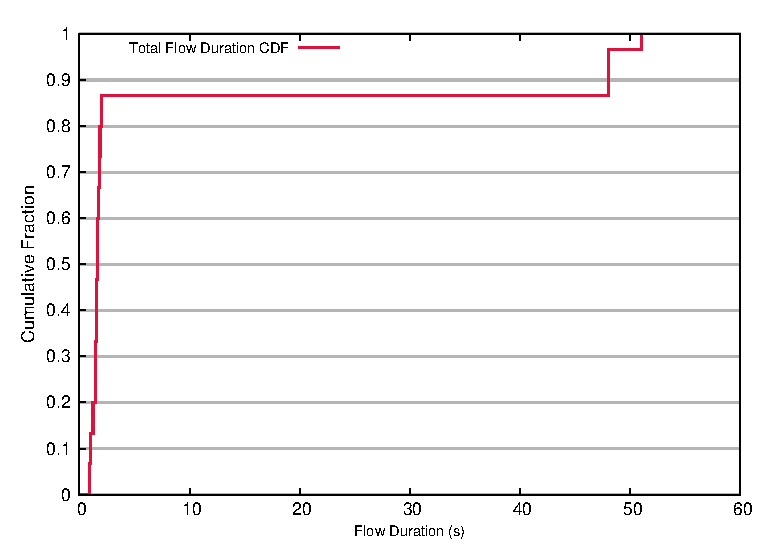
\includegraphics[width=.99\textwidth]{figures/replica_change/flow_duration.eps}
	\caption{All Traffic}\label{fig:read_duration:all}
   \end{subfigure}%
\caption{Replciation Level Change Flow Duration Distribution}
\label{fig:replica_duration}
\end{figure*}

The flow duration distribution of the replication level change workload in figure \ref{fig:replica_duration} exhibit the same characteristics, except for that there is fewer data transfered, thus flows are generally shorter. 


